\documentclass[letterpaper,12pt]{article}
\usepackage{array}
\usepackage{geometry}
\geometry{letterpaper,tmargin=1in,bmargin=1in,lmargin=1.25in,rmargin=1.25in}
%\renewcommand\headrulewidth{0pt}
%\renewcommand\footrulewidth{0pt}
\usepackage{amsmath}
\usepackage{amssymb}
\usepackage{amsthm}
\usepackage{enumerate}
%\usepackage{harvard}
%\usepackage{setspace}
\usepackage{float,color}
\usepackage[pdftex]{graphicx}
\usepackage{hyperref}
\hypersetup{colorlinks,linkcolor=red,urlcolor=blue}
\theoremstyle{definition}
\newtheorem{theorem}{Theorem}
\newtheorem{acknowledgement}[theorem]{Acknowledgement}
\newtheorem{algorithm}[theorem]{Algorithm}
\newtheorem{axiom}[theorem]{Axiom}
\newtheorem{case}[theorem]{Case}
\newtheorem{claim}[theorem]{Claim}
\newtheorem{conclusion}[theorem]{Conclusion}
\newtheorem{condition}[theorem]{Condition}
\newtheorem{conjecture}[theorem]{Conjecture}
\newtheorem{corollary}[theorem]{Corollary}
\newtheorem{criterion}[theorem]{Criterion}
\newtheorem{definition}[theorem]{Definition}
\newtheorem{derivation}{Derivation} % Number derivations on their own
\newtheorem{example}[theorem]{Example}
\newtheorem{exercise}[theorem]{Exercise}
\newtheorem{lemma}[theorem]{Lemma}
\newtheorem{notation}[theorem]{Notation}
\newtheorem{problem}[theorem]{Problem}
\newtheorem{proposition}{Proposition} % Number propositions on their own
\newtheorem{remark}[theorem]{Remark}
\newtheorem{solution}[theorem]{Solution}
\newtheorem{summary}[theorem]{Summary}
%\numberwithin{equation}{section}
\bibliographystyle{aer}
\newcommand\ve{\varepsilon}
\newcommand\boldline{\arrayrulewidth{1pt}\hline}


\begin{document}

\begin{flushleft}
   \textbf{\large{Problem Set \#3}} \\
   MACS 40000, Dr. Evans \\
   Alexandre Sollaci
\end{flushleft}

\vspace{5mm}

\noindent\begin{enumerate}
   \item \textbf{Fitting elliptical disutility of labor to CFE function}
 	\begin{enumerate}[(a)]
 	\item ]In the CFE case, we have
 	\[ v'_{cfe}(l) = (1-l)^{\frac{1}{\theta}} .\]
 	In the elliptical case, 
 	\[ v'_{elp}(l) = b\left[1 - (1-l)^{\mu}\right]^{\frac{1-\mu}{\mu}} (1-l)^{\mu - 1}\]
 	\item My estimates were $b = 0.501$ and $\mu = 1.554$. The plot of the two marginal utilities can be found in figure 1.
 	\end{enumerate}
	
	\item \textbf{Checking feasibility in the steady-state}
	
	\begin{enumerate}[(a)]
	\item The consumption constraint is violated. Specifically, $c_1 < 0$.
	\item Similarly to the case above, the consumption constraint is violated once more. This time $c_2 < 0$.
	\item In this case, none of the constraints are violated.
	\item Once again, none of the constraints are violated.
	\item As a thumb rule, high values for the labor supply and low (but positive) values for savings will not violate any of the constraints.
	\end{enumerate}
	
	\item \textbf{Solve for the steady-state equilibrium}

	\begin{enumerate}[(a)]
	\item The steady state values are
	\begin{verbatim}
{'C_ss': 4.3347304222925924,
 'EulErr_ss': array([ 3.37152511, -2.56403131, -2.19710288, ..., 
 			 2.62509299, 2.67743804,  3.31542748]),
 'K_ss': 1.9763389650259522,
 'L_ss': 8.2417330233076775,
 'RCerr_ss': 5.5511151231257827e-16,
 'Y_ss': 4.999925738767649,
 'b_ss': array([ 0.04176371,  0.10345494,  0.16777769,  0.22660614,  
         0.28004111, 0.32058685,  0.33238941,  0.29556384,  0.20815528]),
 'c_ss': array([ 0.35215818,  0.34907219,  0.37643968,  0.40719693, 
         0.43346902, 0.46243928,  0.48020632,  0.4981081 , 0.49906487,
         0.47657586]),
 'n_ss': array([ 0.9989684 ,  0.98354507,  0.97375055,  0.94828273,  
         0.91934412, 0.88574648,  0.80147411,  0.70712497,  0.63253415, 
         0.39096245]),
 'r_ss': 0.54888291497069996,
 'ss_time': 0.015906726519233416,
 'w_ss': 0.39432868317962816}
	\end{verbatim}
	\item The distribution of consumption and savings is in figure 2; the distribution of labor supply is in figure 3.
	\item When $\alpha$ drops to 0.25, wages increase, since the marginal product of labor has increased. The increase in wages increases the labor supply, increasing $L$. It also makes consumers richer, so consumption increases and so does aggregate production. Savings drop as a higher fraction of consumer's wealth comes from labor. Despite the decrease in $\alpha$, making capital less valuable for production, the increase in $L$ and in total production end up increasing the marginal product of capital, thus increasing the interest rate as well. 
	
The new steady state values are as below:
	\begin{verbatim}
{'C_ss': 5.4922493741343672,
 'K_ss': 1.6744890292626833,
 'L_ss': 9.2954952934901325,
 'Y_ss': 6.0558481694147988,
 'b_ss': array([ 0.02596725,  0.09787919,  0.17396547,  0.24743017,  
         0.31016607, 0.29233795,  0.28944248,  0.18709221,  0.05020824]),
 'c_ss': array([ 0.43384328,  0.43078356,  0.46165551,  0.5045682 ,  
         0.53112749, 0.59709924,  0.63608323,  0.69120299, 0.64256411,  
         0.56332176]),
 'n_ss': array([ 0.94105545,  0.9986618 ,  0.98685773,  0.98093893,  
         0.92800383, 0.82526723,  0.95632237,  0.86894888,  0.81761307,  
         0.99182601]),
 'r_ss': 0.56755417949303399,
 'ss_time': 0.010697268452076969,
 'w_ss': 0.48861152457813578}
	\end{verbatim}
	\end{enumerate}
	
	\item \textbf{Solve for the non-steady-state equilibrium time path}
	
	\begin{enumerate}[(a)]
	\item The plots are in figures 4 (capital), 5 (interest rate) and 6 (wages).
	\item See figures 7 (labor supply) and 8 (savings)
	\end{enumerate}
\end{enumerate}

\clearpage
\section*{Figures}

\begin{figure}[h!]
	\centering
	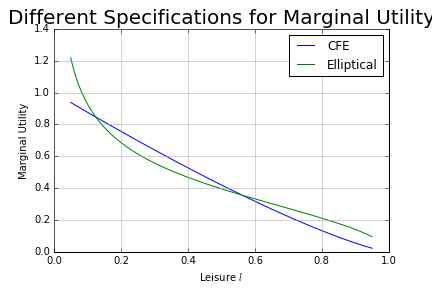
\includegraphics[scale=.8]{code/images/utility_leisure}
	\caption{Marginal utility of leisure in CFE and Elliptical specifications.}
	\end{figure}

\begin{figure}[h!]
	\centering
	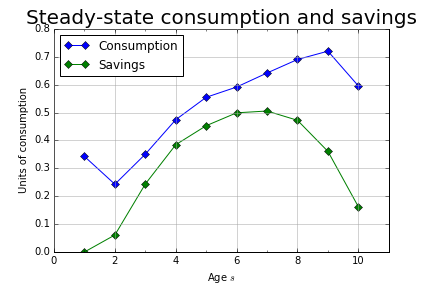
\includegraphics[scale=.8]{code/images/SS_bc}
	\caption{Distribution of consumption and savings in steady state.}
	\end{figure}
	
	\begin{figure}[h!]
	\centering
	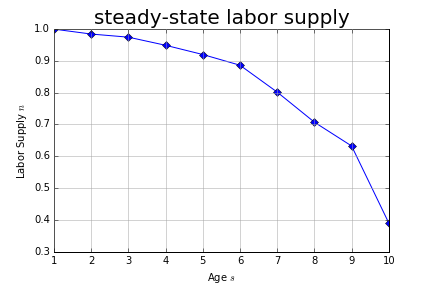
\includegraphics[scale=.8]{code/images/SS_n}
	\caption{Distribution of labor supply in steady state.}
	\end{figure}
	
	\begin{figure}[h!]
	\centering
	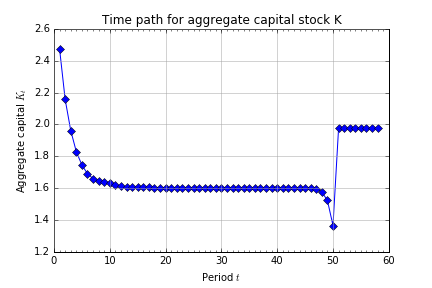
\includegraphics[scale=.8]{code/images/Kpath}
	\caption{Time path of capital to Steady State.}
	\end{figure}
	
	\begin{figure}[h!]
	\centering
	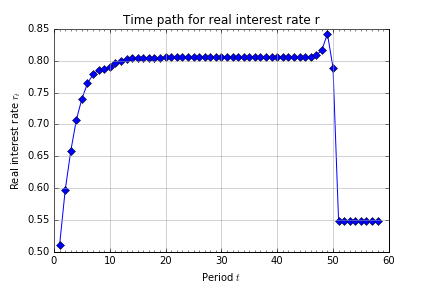
\includegraphics[scale=.8]{code/images/rpath}
	\caption{Time path of interest rate to Steady State.}
	\end{figure}

	\begin{figure}[h!]
	\centering
	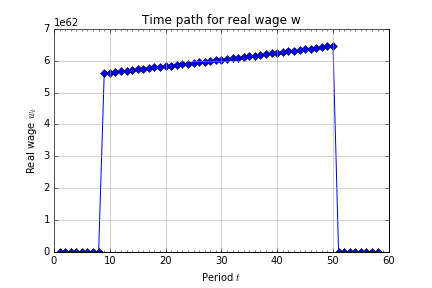
\includegraphics[scale=.8]{code/images/wpath}
	\caption{Time path of wages to Steady State.}
	\end{figure}
	
	\begin{figure}[h!]
	\centering
	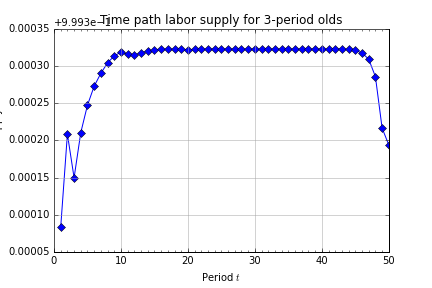
\includegraphics[scale=.8]{code/images/tpi_n}
	\caption{Equilibrium time path labor supply for 3-period olds.}
	\end{figure}
	
	\begin{figure}[h!]
	\centering
	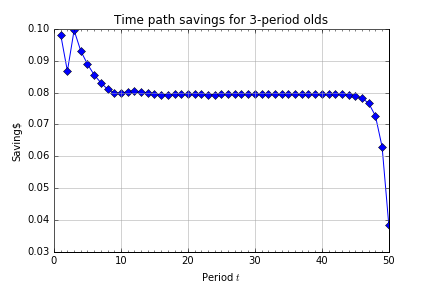
\includegraphics[scale=.8]{code/images/tpi_s}
	\caption{Equilibrium time path savings for 3-period olds.}
	\end{figure}

\end{document}





